\documentclass[letterpaper]{article} % DO NOT CHANGE THIS
\usepackage[submission]{aaai24}  % DO NOT CHANGE THIS
\usepackage{times}  % DO NOT CHANGE THIS
\usepackage{helvet}  % DO NOT CHANGE THIS
\usepackage{courier}  % DO NOT CHANGE THIS
\usepackage[hyphens]{url}  % DO NOT CHANGE THIS
\usepackage{graphicx} % DO NOT CHANGE THIS
\urlstyle{rm} % DO NOT CHANGE THIS
\def\UrlFont{\rm}  % DO NOT CHANGE THIS
\usepackage{natbib}  % DO NOT CHANGE THIS AND DO NOT ADD ANY OPTIONS TO IT
\usepackage{caption} % DO NOT CHANGE THIS AND DO NOT ADD ANY OPTIONS TO IT
\frenchspacing  % DO NOT CHANGE THIS
\setlength{\pdfpagewidth}{8.5in} % DO NOT CHANGE THIS
\setlength{\pdfpageheight}{11in} % DO NOT CHANGE THIS
%
% These are recommended to typeset algorithms but not required. See the subsubsection on algorithms. Remove them if you don't have algorithms in your paper.
\usepackage{algorithm}
\usepackage{algorithmic}

%
% These are are recommended to typeset listings but not required. See the subsubsection on listing. Remove this block if you don't have listings in your paper.
\usepackage{newfloat}
\usepackage{listings}

% User imported packages
\usepackage{multirow}
\usepackage{pifont}
\usepackage{booktabs}
\usepackage{subcaption}
\usepackage{bm}
\usepackage{amsmath}
\usepackage{amssymb}
\usepackage{cleveref}
\usepackage{todonotes}
\usepackage{varwidth}
\usepackage{tikz}
\usepackage{graphicx}
\newcommand{\cmark}{\ding{51}} % checkmark symbol
\newcommand{\xmark}{\ding{55}} % X-mark symbol

\DeclareCaptionStyle{ruled}{labelfont=normalfont,labelsep=colon,strut=off} % DO NOT CHANGE THIS
\lstset{%
	basicstyle={\footnotesize\ttfamily},% footnotesize acceptable for monospace
	numbers=left,numberstyle=\footnotesize,xleftmargin=2em,% show line numbers, remove this entire line if you don't want the numbers.
	aboveskip=0pt,belowskip=0pt,%
	showstringspaces=false,tabsize=2,breaklines=true}
\floatstyle{ruled}
\newfloat{listing}{tb}{lst}{}
\floatname{listing}{Listing}
%
% Keep the \pdfinfo as shown here. There's no need
% for you to add the /Title and /Author tags.
\pdfinfo{
/TemplateVersion (2024.1)
}

% DISALLOWED PACKAGES
% \usepackage{authblk} -- This package is specifically forbidden
% \usepackage{balance} -- This package is specifically forbidden
% \usepackage{color (if used in text)
% \usepackage{CJK} -- This package is specifically forbidden
% \usepackage{float} -- This package is specifically forbidden
% \usepackage{flushend} -- This package is specifically forbidden
% \usepackage{fontenc} -- This package is specifically forbidden
% \usepackage{fullpage} -- This package is specifically forbidden
% \usepackage{geometry} -- This package is specifically forbidden
% \usepackage{grffile} -- This package is specifically forbidden
% \usepackage{hyperref} -- This package is specifically forbidden
% \usepackage{navigator} -- This package is specifically forbidden
% (or any other package that embeds links such as navigator or hyperref)
% \indentfirst} -- This package is specifically forbidden
% \layout} -- This package is specifically forbidden
% \multicol} -- This package is specifically forbidden
% \nameref} -- This package is specifically forbidden
% \usepackage{savetrees} -- This package is specifically forbidden
% \usepackage{setspace} -- This package is specifically forbidden
% \usepackage{stfloats} -- This package is specifically forbidden
% \usepackage{tabu} -- This package is specifically forbidden
% \usepackage{titlesec} -- This package is specifically forbidden
% \usepackage{tocbibind} -- This package is specifically forbidden
% \usepackage{ulem} -- This package is specifically forbidden
% \usepackage{wrapfig} -- This package is specifically forbidden
% DISALLOWED COMMANDS
% \nocopyright -- Your paper will not be published if you use this command
% \addtolength -- This command may not be used
% \balance -- This command may not be used
% \baselinestretch -- Your paper will not be published if you use this command
% \clearpage -- No page breaks of any kind may be used for the final version of your paper
% \columnsep -- This command may not be used
% \newpage -- No page breaks of any kind may be used for the final version of your paper
% \pagebreak -- No page breaks of any kind may be used for the final version of your paperr
% \pagestyle -- This command may not be used
% \tiny -- This is not an acceptable font size.
% \vspace{- -- No negative value may be used in proximity of a caption, figure, table, section, subsection, subsubsection, or reference
% \vskip{- -- No negative value may be used to alter spacing above or below a caption, figure, table, section, subsection, subsubsection, or reference

\setcounter{secnumdepth}{2} %May be changed to 1 or 2 if section numbers are desired.

% The file aaai24.sty is the style file for AAAI Press
% proceedings, working notes, and technical reports.
%

% Title

% Your title must be in mixed case, not sentence case.
% That means all verbs (including short verbs like be, is, using,and go),
% nouns, adverbs, adjectives should be capitalized, including both words in hyphenated terms, while
% articles, conjunctions, and prepositions are lower case unless they
% directly follow a colon or long dash
\iffalse\title{AAAI Press Anonymous Submission\\Instructions for Authors Using \LaTeX{}}
\author{
    %Authors
    % All authors must be in the same font size and format.
    Written by AAAI Press Staff\textsuperscript{\rm 1}\thanks{With help from the AAAI Publications Committee.}\\
    AAAI Style Contributions by Pater Patel Schneider,
    Sunil Issar,\\
    J. Scott Penberthy,
    George Ferguson,
    Hans Guesgen,
    Francisco Cruz\equalcontrib,
    Marc Pujol-Gonzalez\equalcontrib}
\affiliations{
    %Afiliations
    \textsuperscript{\rm 1}Association for the Advancement of Artificial Intelligence\\
    % If you have multiple authors and multiple affiliations
    % use superscripts in text and roman font to identify them.
    % For example,

    % Sunil Issar\textsuperscript{\rm 2},
    % J. Scott Penberthy\textsuperscript{\rm 3},
    % George Ferguson\textsuperscript{\rm 4},
    % Hans Guesgen\textsuperscript{\rm 5}
    % Note that the comma should be placed after the superscript

    1900 Embarcadero Road, Suite 101\\
    Palo Alto, California 94303-3310 USA\\
    % email address must be in roman text type, not monospace or sans serif
    proceedings-questions@aaai.org
%
% See more examples next
}
\fi

%Example, Single Author, ->> remove \iffalse,\fi and place them surrounding AAAI title to use it
\iffalse\title{My Publication Title --- Single Author}
\author{
    Author Name
}
\affiliations{
    Affiliation\\
    Affiliation Line 2\\
    name@example.com
}
\fi

%Example, Multiple Authors, ->> remove \iffalse,\fi and place them surrounding AAAI title to use it
\title{Learning Rate Optimization in Online Deep Learning}
\author{
    % Authors
    Lucas Cazzonelli\textsuperscript{\rm 1},
    Cedric Kulbach\textsuperscript{\rm 2},
}
\affiliations{
    % Affiliations
    \textsuperscript{\rm 1}FZI Research Center for Information Technology\\
    \textsuperscript{\rm 2}Affiliation 2\\
    cazzonelli@fzi.de, secondAuthor@affilation2.com
}


% REMOVE THIS: bibentry
% This is only needed to show inline citations in the guidelines document. You should not need it and can safely delete it.
\usepackage{bibentry}
% END REMOVE bibentry

\begin{document}

\maketitle
% \frenchspacing

\begin{abstract}
	\noindent Efficient training via gradient-based optimization techniques is an essential building block to the success of deep learning. Extensive research on the impact and the effective estimation of an appropriate learning rate has partly enabled these techniques. Despite the proliferation of data streams generated by IoT devices, digital platforms, etc., previous research has been primarily focused on batch learning, which assumes that all training data is available a priori. However, characteristics such as the gradual emergence and non-stationarity of data pose additional challenges. Therefore, the findings on batch learning may not be applicable to deep learning in streaming environments. In this work, we seek to address this knowledge gap by (i) evaluating and comparing typical learning rate schedules and optimizers, (ii) exploring adaptations of these techniques, and (iii) providing insights into effective learning rate tuning in the context of stream-based deep learning.
\end{abstract}

\section{Introduction}
Deep learning models have demonstrated exceptional performance in various domains.
One of the main factors leading to such outstanding results is the choice of the optimization method used to train the target model.
Nearly all modern deep learning applications, use first-order stochastic optimization methods like \text{stochastic gradient descent}, which iteratively update the parameters of the underlying model based on gradient information, for this purpose.
One of the most important variables of such algorithms is the step size or \textit{learning rate} (LR).

As a result, many techniques for setting and optimizing the learning rate have emerged over the years (see Figure~\ref{fig:lr_overview}).
Based on prior knowledge, the learning rate can for instance be set as a fixed value or a schedule altering the step size over time.
Alternatively, one could use an adaptive learning rate technique, which considers historical gradient information to modify the learning rate at each iteration.

In batch learning scenario where all training data is assumed to be available a priori, the aforementioned methods are well researched.
Despite the increasing prevalence of data streams, their use in online learning has however received little attention in research.

According to \citet{bifetMOAMassiveOnline2010} an online learning model operating on a data stream must be able to
\begin{center}
	\begin{varwidth}{0.5\textwidth}
		\begin{description}
			\item[R1:] process a single instance at a time,\label{rq:single_instance}
			\item[R2:] process each instance in a limited amount of time,\label{rq:limited_time}
			\item[R3:] use a limited amount of memory,\label{rq:limited_memory}
			\item[R4:] predict at any time,\label{rq:predict_any_time}
			\item[R5:] adapt to changes in the data distribution.\label{rq:adapt_to_drift}
		\end{description}
	\end{varwidth}
\end{center}

These requirements introduce additional challenges when it comes to the selection of an appropriate optimizer and learning rate.

To enable more informed decisions when it comes to learning rate optimization, we provide insight into these challenges and empirically evaluate commonly used optimization techniques in an online learning setting (i).
We further introduce a \textit{drift reset} mechanism to adapt the learning rate to concept drifts, that commonly occur in streaming environments (ii).
Lastly, we propose a \textit{pre-tuning} approach for effectively optimizing the learning rate of online deep learning models \textit{pre-stream} (see Figure~\ref{fig:lr_overview}) (iii).

\begin{figure}
	\centering
	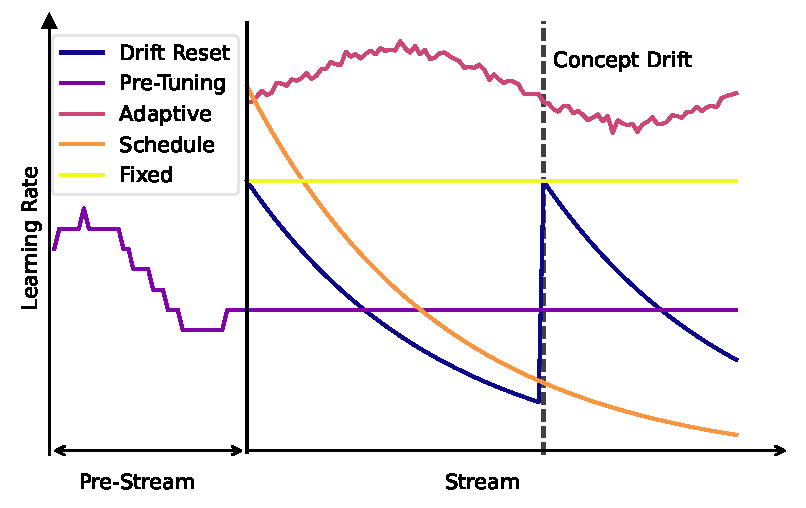
\includegraphics[width=0.45\textwidth]{figures/lr_overview.pdf}
	\caption{Overview of different learning rate optimization approaches.}
	\label{fig:lr_overview}
\end{figure}

\section{Learning Rate in First-Order Optimization}

In the following, we will explain the theoretical background of first-order stochastic optimization enabling modern deep learning models.
We will also outline the differences between the application of these techniques in traditional batch learning and online learning in terms of impact of the learning rate and its optimization.

First-order stochastic optimization algorithms like stochastic gradient descent typically aim to solve
\begin{equation}
	\min_{\theta} \mathbb{E}_{x \sim p(x)} [\mathcal{L}(x, \theta)],
\end{equation}
where $\mathcal{L}(x, \theta)$ represents a loss function that quantifies the predictive error of the model given a mini-batch of data samples $x$ and model parameters $\theta$.
The blueprint process of solving this problem via first order stochastic optimization consists of the following steps for each iteration $t \in 0, \ldots, T$:
\begin{enumerate}
	\item Draw a mini-batch of samples $x_t$ from distribution $p(x)$.
	\item Calculate the loss $\mathcal{L}_t = \mathcal{L}(x_t, \theta_t)$ for $x_t$ and current parameters $\theta_t$.
	\item Compute the gradient $g_t = \nabla_{\theta_t} \mathcal{L}_t$ with respect to the parameters.
	\item Update the parameters for the next iteration using $g_t$ and potentially information from past iterations.
\end{enumerate}

For basic SGD, we can define the parameter update performed at the end of each iteration as
\begin{equation}
	\theta_{t}  = \theta_{t} - \eta_t \cdot g_t,
\end{equation}
where $\eta_t$ denotes the step size or \textit{learning rate} at timestep $t$.

The primary trade-off to consider with respect to the choice of $\eta$ is that increasing it speeds up convergence, but at the same time also increases stochasticity and therefore leads to the divergence of the training criterion beyond a certain threshold.~\cite{bengioPracticalRecommendationsGradientbased2012}.
In fact, \citet{smithBayesianPerspectiveGeneralization2018}, found that when modeling SGD as a stochastic differential equation, the “noise scale” is directly tied to $\eta$~\cite{smithBayesianPerspectiveGeneralization2018}.

\subsection{Learning Rate Schedules}

While using a single fixed learning rate $\eta_t = \eta$ for all iterations simplifies the learning selection and can often yield sufficient performance, results can generally be improved with a schedule with step sizes specific to each iteration~\cite{wuDemystifyingLearningRate2019b}.
To ensure fast convergence at the start of training, while mitigating jumping around potential minima at later stages it is, for instance, common to use a decaying schedule starting with a large learning rate that decreases over time.
An additional benefit of this approach is that of potentially better generalization, since larger learning rates may help skipping over sharp minima with poor generalization~\cite{hochreiterFlatMinima1997,chaudhariEntropySGDBiasingGradient2017}.
Some have likened this procedure to simulated annealing, which shifts its focus from exploration at high temperatures to exploitation once temperatures have sufficiently decreased~\cite{smithDonDecayLearning2018}.

Commonly used forms of decay are exponential decay, where $\eta_{t}$ calculates as
$\eta_{t} = \eta_0 \cdot \gamma^t$,
% \begin{equation}
% 	\eta_{t} = \eta_0 \cdot \gamma^t,
% \end{equation}
with $\gamma < 1$, and stepwise decay, which for a regular interval between steps of length $s$ is given as $\eta_0 \cdot \gamma^{\lfloor t/s \rfloor}$.
% \begin{equation}
% 	\eta_{t} = \eta_0 \cdot \gamma^{\lfloor t/s \rfloor}.
% \end{equation}
Another common approach involves decaying $\eta$ every time the training loss plateaus for a set number of iterations.

Other popular schedules include cyclic learning rates which oscillate $\eta$ between two values over a predefined interval.
For a triangular cycle, the learning rate calculates as
\begin{equation}
	\eta_t = \eta_0 + \frac{\hat{\eta} - \eta_0}{2s} \cdot \min_{i} \{|t-i\cdot s|\},
\end{equation}
with $\hat{\eta}$ being the learning rate at the middle of each cycle of length $s$.
Some studies~\cite{smithCyclicalLearningRates2017, smithSuperConvergenceVeryFast2018a} have found cyclic schedules to significantly speed up the convergence of neural networks even when compared to adaptive techniques like Adam in some cases~\cite{kingmaAdamMethodStochastic2017b}.
While there are many alternatives, in this work we focus on  exponential, stepped and cyclic learning rates, as some of the most commonly used generic schedules.
For a comprehensive overview and detailed analysis on learning rate policies, refer to \citet{wuDemystifyingLearningRate2019b}.

\subsection{Adaptive Learning Rates}

Although determining the learning rate through a separate tuning phase with parameter searches like grid- or random-search is still the de facto standard in deep learning~\cite{defazioLearningRateFreeLearningDAdaptation2023a}, this approach causes significant computational overhead.

To decrease such computational overhead, various studies have proposed \textit{adaptive optimizers}.
These optimizers adjust the learning rate by considering additional loss landscape information from the previous gradients at each optimization step, enhancing their robustness with respect to the learning rate~\cite{duchiAdaptiveSubgradientMethods2011}.

One of the earlier optimizers in this category is \textit{AdaGrad}~\cite{duchiAdaptiveSubgradientMethods2011}, which scales the learning rate based on the sum of squares of past gradients for each parameter, resulting in a parameter specific step size.
Unlike a global value, parameter specific learning rates not only influence the length, but also the direction of update steps, in case of AdaGrad by shifting updates in the direction of smaller gradients~\cite{wuWNGradLearnLearning2020}. % Weglassen? 

Several other approaches like AdaDelta~\cite{zeilerADADELTAAdaptiveLearning2012a} and RMSProp~\cite{tielemanLecture5rmspropDivide2012}, subsequently built on AdaGrad's scaling approach.
The same applies to the commonly used Adam optimizer~\cite{kingmaAdamMethodStochastic2017b}, that additionally takes a momentum term of past gradients
% ~\cite{sutskeverImportanceInitializationMomentum2013} 
into account to speed up the convergence for parameters with consistent derivatives.

Another optimizer building on AdaGrad is \textit{WNGrad}~\cite{wuWNGradLearnLearning2020}, which adaptively scales each parameter update based on the squared sum of past gradients.
By doing so, WNGrad achieves a step size robust global learning rate~\cite{wuWNGradLearnLearning2020}.

Adaptive approaches such as AdaGrad and Adam have been shown to reduce dependence on the learning rate, but often times still require manual tuning~\cite{wuWNGradLearnLearning2020}.
Parameter-free variants of SGD aim to solve this by estimating the optimal step size online as training progresses, thus eliminating the learning rate entirely.

One of the earlier works on parameter-free optimization~\cite{schaulNoMorePesky2013} proposed \textit{vSGD}, which, like Adam, uses first and second order moments of the gradients as well as local curvature information to estimate $\eta$~\cite{schaulNoMorePesky2013} obtained through a back-propagation formula~\cite{schaulNoMorePesky2013}.
Due to the age and complexity of vSGD compared to similar approaches, we did not include it in our evaluations.
% Even though \citet{schaulNoMorePesky2013} demonstrate \textit{vSGD's} robustness to non-stationary data distributions, it has, to the best of our knowledge, not been widely adopted in the online learning space.
% Due to the lack of publicly available implementations of the non-trivial algorithm, we have not been able to evaluate vSGD at the time of writing. 

Instead of using curvature information, the \textit{COCOB} algorithm~\cite{orabonaTrainingDeepNetworks2017} models parameter optimization as a gambling problem, in which the goal is to maximize the rewards obtained from betting on each gradient.
The resulting strategy corresponds to running a meta optimization algorithm, that estimates the expected optimal learning rate~\cite{orabonaTrainingDeepNetworks2017}.

Several other contributions~\cite{vanervenMetaGradMultipleLearning2016a,baydinOnlineLearningRate2018,cutkoskyMechanicLearningRate2023} have also used the idea of learning $\eta$ via a meta-optimization process.
The \textit{hypergradient descent} (HD) approach~\cite{baydinOnlineLearningRate2018} for instance adapts the learning rate of a base optimizers like SGD using a meta-gradient descent procedure, although this does not remove the learning rate completely but replaces it with a less sensitive hypergradient step size.
Mechanic~\cite{cutkoskyMechanicLearningRate2023} pursues the same goal using a meta \textit{online convex optimization} (OCO) algorithm to estimate the step size of an arbitrary base optimizer.

Research has shown that in an OCO problem setting with stationary data, the worst-case optimal fixed step size for SGD is
\begin{equation}\label{eq:oco_optimal_lr}
	\eta^* = \frac{||\theta_0 - \theta^*||}{\sqrt{\sum_{t=0}^{T} ||g_t||^2}}.
\end{equation}
Multiple recently introduced parameter-free optimizers, have made use of this result.
As its name suggests, the \textit{Distance over Gradients} (DoG)~\cite{ivgiDoGSGDBest2023} algorithm estimates the unknown numerator in Equation~\ref{eq:oco_optimal_lr} as the maximum distance between the initial parameters and the parameters of all previous iterations
\begin{equation}
	\max_{i<t}||\theta_0 - \theta_i||.
\end{equation}
DoG additionally makes use of polynomial decay averaging as proposed by~\citet{shamirStochasticGradientDescent2012}.

\textit{D-Adaptation} by \citet{defazioLearningRateFreeLearningDAdaptation2023a} on the other hand employs weighted dual averaging~\cite{duchiDualAveragingDistributed2012} to calculate bounds on the distance between initial and optimal parameters, often denoted as $D$ and use them to adapt the learning rate of a base optimization algorithm.

Although parameter-free stochastic optimization techniques are inherently well-suited for highly non-stationary streaming data~\cite{schaulNoMorePesky2013} and in some cases even developed as online optimizers, their application on data streams has rarely been investigated.
Therefore, we assess the suitability of some of the most prominent adaptive optimizers, listed in Table~\ref{tab:param_free_optims} for stream-based learning.

There are also several lesser-known studies that have explored adaptive learning rates in specific application domains of online learning such as time series prediction~\cite{miyaguchiCograConceptDriftAwareStochastic2019, fekriDeepLearningLoad2021}, federated learning~\cite{canonacoAdaptiveFederatedLearning2021}, and recommender systems~\cite{ferreirajoseADADRIFTAdaptiveLearning2020}.
However, since we focus on general data stream applications in this paper, we did not investigate these techniques further.

\begin{table}[ht]
	\centering
	\small
	\begin{tabular}{@{}lllcc@{}}
		\toprule
		Optimizer                & Runtime            & Space             & Param. specific & LR free \\ \midrule
		AdaGrad                  & $\mathcal{O}(5D)$  & $\mathcal{O}(1D)$ & \cmark          & \xmark  \\
		Adam                     & $\mathcal{O}(12D)$ & $\mathcal{O}(2D)$ & \cmark          & \xmark  \\
		WNGrad                   & $\mathcal{O}(2D)$  & $\mathcal{O}(0)$  & \xmark          & \xmark  \\
		COCOB                    & $\mathcal{O}(14D)$ & $\mathcal{O}(4D)$ & \cmark          & \cmark  \\
		HD \footnotemark[1]      & $\mathcal{O}(2D)$  & $\mathcal{O}(1D)$ & \xmark          & \xmark  \\
		Mechanic                 & $\mathcal{O}(10D)$ & $\mathcal{O}(1D)$ & \cmark          & \cmark  \\
		DoG \footnotemark[1]     & $\mathcal{O}(5D)$  & $\mathcal{O}(1D)$ & \xmark          & \cmark  \\
		D-Adapt \footnotemark[1] & $\mathcal{O}(6D)$  & $\mathcal{O}(2D)$ & \xmark          & \cmark  \\
		% vSGD      & $\mathcal{O}(21D)$\footnotemark & $\mathcal{O}(4D)$ & \cmark          & \cmark  \\ % Remove since not evaluated?
		\bottomrule
	\end{tabular}
	\caption{Overview of additional time- and space-complexity of evaluated adaptive first-order optimizers compared to basic SGD. Values are given in big O notation with respect to the number of model parameters $D$ and based on pseudo-codes provided in the original works. Note that this is not a comprehensive list.}\label{tab:param_free_optims}
\end{table}
\footnotetext[1]{Variant with SGD as the base algorithm.}

\section{Differences between Batch and Online Learning}\label{sec:diffs_batch_online}

In a batch learning setting, optimizing the learning rate involves minimizing the expected loss on a hold-out set of validation data.
Formally, we can denote this task as
\begin{equation}
	\label{eq:batch_lr_optim}
	\min_{\eta_0, \ldots, \eta_T} \mathbb{E}_{x \sim p_v(x)}[\mathcal{L}(x, \theta_T)],
\end{equation}
where $p_v$ is a distribution of held-out validation data and $\theta_T$ the parameters at the end of training.
% , which for basic SGD are given by
% \begin{equation}
% 	\theta_T = \sum_{t=0}^{T} \eta_t \cdot g_t.
% \end{equation}
In online learning where data is generated incrementally, this notion of learning rate optimization is infeasible.
Due to requirements \textbf{R1-R5}, models operating in an online learning environment should be evaluated in a \textit{prequential} manner~\cite{bifetMOAMassiveOnline2010}, where each sample $x_t$ in the data stream is first used to test and then to train the model ensuring testing is done exclusively on unseen data.

Training in such a scenario can therefore be more accurately modeled as an online convex optimization problem~\cite{shalev-shwartzOnlineLearningOnline2011,hazanIntroductionOnlineConvex2016}, where the optimizer suffers a loss $\mathcal{L}_t(\theta_t) = \mathcal{L}(x_t, \theta_{t})$ and produces updated parameters $\theta_{t+1}$ at each iteration of the data stream.
The task of finding an optimal learning rate schedule in this setting can be formulated as
\begin{equation}
	\label{eq:stream_lr_optim}
	\min_{\eta_0, \ldots, \eta_T} \sum_{t=0}^{T} \mathcal{L}_t(\theta_t).
\end{equation}

Compared to Equation~\eqref{eq:batch_lr_optim}, Equation~\eqref{eq:stream_lr_optim} features some key differences.
Due to the requirement of being able to predict at any time (\textbf{R4}), the goal is to minimize the total sum of losses incurred over all timesteps of the prequential evaluation process, instead of minimizing only the validation loss for the final parameters $\theta_T$.
This means that the loss suffered at every timestep of the stream contributes equally to the objective.
Therefore, the speed of convergence is more important in the streaming setting, while the performance of the final $\theta_T$ parameter has relatively little impact.
Since memory is limited (Requirement~\ref{rq:limited_memory}), it is also not possible to continue training on previously observed data as long as $\mathcal{L}$ decreases, which puts an even greater emphasis on quick adaptation.
At the same time, a larger learning rate causing temporary loss increases, due to skipping over local minima can be suboptimal with respect to Equation~\eqref{eq:stream_lr_optim} even if it eventually yields a lower loss.

Another difference to conventional batch learning is that the loss function $\mathcal{L}_t$ is time dependent, due to the fact that data streams are commonly subjected to change in the form of \textit{concept drift} over time.
Under such circumstances, the optimal parameter values $\theta^*$ move throughout the progression of the stream requiring the model parameters to adapt.

\subsection{Learning Rate Tuning}\label{subsec:pre-tuning}

Tuning the learning rate of an online machine learning model is a challenging task owing to the possibility of concept drift that may cause data stream to move away from the distribution used for tuning the model.
This effect, combined with the previously described differences in the evaluation scheme may cause conventional learning rate tuning to produce unsuitable results for stream-based learning.
We therefore propose a modified tuning approach, approximating Equation~\eqref{eq:stream_lr_optim}, which we call learning rate \textit{pre-tuning} in the following.

To emulate
% a static version of 
the targeted data stream we continually draw samples with replacement from the tuning data in a bootstrapping procedure instead of training on all data for multiple epochs.
By doing so we aim to increase data variability, and therefore the resemblance to an actual data stream with random distributional shifts.
We then optimize $\eta$ with respect to the mean prequential performance over the emulated stream instead of the performance on a validation set.
For this purpose we use a basic grid-search as is customary in batch learning~\cite{defazioLearningRateFreeLearningDAdaptation2023a}.
We provide a detailed experimental evaluation of our approach in Section~\ref{sec:experiments}.

\subsection{Learning Rate Adaptation}

As previously noted, concept drift requires the model parameters to repeatedly adapt.
When interpreting the post-drift training as a new online optimization problem, the worst-case optimal learning rate can be calculated according to Equation~\ref{eq:oco_optimal_lr} substituting the initial parameter values $\theta_0$ with the values at the time of drift onset $\theta_{t_d}$.
As a result, more severe drifts, causing $\theta^*$ to move away from $\theta_{t_d}$, may benefit from larger learning rates.

Based on this notion, \citet{kunchevaAdaptiveLearningRate2008} introduced an adaptive schedule that uses the predictive losses as an indicator for concept drift.
Their approach updates the learning rate using
\begin{equation}
	\eta_{t+1} = \eta_t^{1+	\bar{\mathcal{L}}_{t-M} - \bar{\mathcal{L}}_{t}},
\end{equation}\label{eq:kuncheva_lr}
where $\bar{\mathcal{L}}_{t}$ is the running mean of $M$ previous losses.
By doing so, the authors aim to achieve higher stability, when losses decline and higher adaptability when losses rise.
While this approach seems intuitively sound, for an initial learning rate $\eta_0 \leq 1$ it can cause an instable learning rate, since increases in loss caused by an excessive learning rate would lead to a feedback loop.
Furthermore, loss plateaus that could be avoided by lowering $\eta$ would instead cause $\eta$ to remain stable, diminishing performance.

To offer the same potential benefits as \citet{kunchevaAdaptiveLearningRate2008} approach while addressing its fundamental issues, we propose a simple adaptation to decaying learning rate schedules that resets $\eta$ to its original value if a concept drift has been detected.
An exponential schedule modified with our approach therefore yield learning rates
\begin{equation}
	\eta_t = \eta_0 \cdot \gamma^{t-t_d},
\end{equation}\label{eq:drift_reset}
where $t_d$ marks the timestep in which drift was last detected.
As a result, feedback-loops are avoided assuming $\eta_0$ is small enough to not cause divergence and $\eta_t$ can also decay in the presence of loss plateaus.
For the purpose of drift detection we apply ADWIN~\cite{bifetLearningTimeChangingData2007} to the prequential losses.
To avoid mistakenly detecting drops in loss as concept drifts, we use a one-tailed ADWIN variant that tests only for increases.

Our approach is similar to some \textit{forgetting mechanisms} commonly employed in conventional non-deep online learning~\cite{gamaSurveyConceptDrift2014}.
To improve model plasticity, such mechanisms partly or completely reset the current model parameters to their initial values.
However, we hypothesize that this approach is not well suited for deep learning purposes.
The reason for this is that, under the assumption of convexity, the newly initiated parameters must be closer to the optimal parameters $\theta^*$ than the current parameters to be beneficial.
For all but the most severe drifts, this seems highly unlikely.
Nevertheless, we experimentally compare our approach with this mechanism in Section~\ref{sec:experiments}.

\section{Experiments}\label{sec:experiments}

To evaluate our hypotheses, we perform computational experiments using the following setup\footnote[2]{Code available at \url{anonymous.4open.science/r/LODL-D458/}.}:

We use both synthetic and publicly available real-world classification datasets with different sizes and types of concept drift, listed in Table~\ref{tab:datasets}.
With the purpose of generating similar datasets with different types of concept drift, we generate \textit{Random Radial Basis Function} (RBF) datasets using the online learning framework \textit{River}~\cite{montiel2021river}. 
We then caused concept drift by incrementally moving data centroids or abruptly switching the random seed of the generator.
We further employ the \textit{Electricity} and \textit{Covertype}~\cite{misc_covertype_31} datasets, which are commonly used to evaluate online learning models, as well as the Insects datasets~\cite{souzaChallengesBenchmarkingStream2020} with known types of concept drift.
\textit{Covertype} is accessible through the \textit{OpenML} Platform~\cite{vanschorenOpenMLNetworkedScience2014}, while the remaining datasets are part of River.

As the model architecture, we use a single hidden layer MLP implemented in \textit{PyTorch}~\cite{paszkePyTorchImperativeStyle2019}.
To account for the different dimensionality of the selected data streams, with the number of hidden units equal to number of input features.
This choice is based on our experience that smaller models exhibit faster convergence and are therefore usually the most suitable in online learning scenarios.

We tune the base learning rate $\eta_0$ of all but the parameter-free approaches using a grid search of ten geometrically spaced values.
To ensure a minimal level of adaptability, we set a lower bound at 10\% of the base learning rate.
Parameter-free algorithms are configured with the author's suggested parameter values and paired with SGD as a base optimizer in the case of HD, Mechanic and D-Adaptation.
We select a fixed factor $\gamma$ for decay schedules on all datasets.
For the proposed learning rate resetting mechanism, we select a smaller decay factor and set the confidence level $\delta$ for drift detection to $10^{-4}$.
For more details on our hyperparameter setup, please refer to Appendix~\ref{app:hyperparams}.
\begin{table}[t]
	\small
	\begin{tabular}{@{}clcccc@{}}
		\toprule
		Type                    & Data Stream               & Instances & Features & Classes \\
		\midrule
		\multirow{2}{*}{Synth.} & RBF abrupt                & 20000     & 20       & 5       \\
		                        & RBF incremental           & 20000     & 20       & 5       \\
		\midrule
		\multirow{5}{*}{Real}   & Insects abrupt            & 52848     & 33       & 6       \\
		                        & Insects incremental       & 57018     & 33       & 6       \\
		                        & Insects gradual           & 24150     & 33       & 6       \\
		                        & Covertype\footnotemark[3] & 100000    & 54       & 7       \\
		                        & Electricity               & 45312     & 8        & 2       \\
		\bottomrule
	\end{tabular}
	\caption{Datasets used for experimental evaluations.}
	\label{tab:datasets}
\end{table}
\footnotetext[3]{We use the first 100k from a total of 581k examples only.}
For our evaluations we process each dataset sequentially, emulating streams of mini-batches with four instances each, while recording the prequential accuracy and other metrics in intervals of 25 iterations.
We report our results averaged over five random seeds.
Since the prequential binary crossentropy used for training occasionally produced large outliers, we focus on the classification accuracy as a performance metric.

\subsection{Drift Adaptation}

\begin{table*}[ht]
	\centering
	\small
	\begin{tabular}{llccccccc}
		\toprule
		                                                    & Schedule        & RBF abrupt            & RBF incr.           & Covertype             & Electricity           & Insects abrupt        & Insects gradual       & Insects incr.         \\
		\midrule
		\multirow{4}{*}{\rotatebox[origin=c]{90}{Static}}   & Fixed           & \underline{94.79±.32} & 70.95±2.89          & \underline{83.42±.50} & \underline{73.77±.40} & 71.50±.08             & 75.31±.21             & 60.48±.20             \\
		                                                    & Step            & \bfseries 94.87±.28   & 70.19±3.02          & 82.89±.37             & \underline{73.62±.53} & \bfseries 72.23±.27   & \underline{75.83±.21} & \underline{61.18±.11} \\
		                                                    & Cyclic          & \underline{94.79±.32} & \bfseries 74.96±.86 & \bfseries 83.44±.08   & 68.38±.81             & 71.74±.39             & 75.64±.06             & 60.48±.20             \\
		                                                    & Exponential     & \underline{94.85±.29} & 70.23±2.40          & 82.95±.26             & \underline{73.51±.48} & \underline{72.19±.37} & \bfseries 75.91±.14   & \bfseries 61.28±.16   \\ \midrule
		\multirow{4}{*}{\rotatebox[origin=c]{90}{Adaptive}} & Weight Reset    & 69.96±.38             & 65.13±.80           & 83.12±.13             & 70.08±1.66            & 51.52±.90             & 62.55±2.34            & 34.11±.44             \\
		                                                    & Kuncheva        & 70.60±6.24            & 42.37±1.31          & 76.98±.15             & 67.06±.01             & 67.45±.50             & 72.43±.61             & 54.17±.30             \\
		                                                    & LR Reset (Ours) & \underline{94.83±.26} & 73.38±2.32          & 82.99±.20             & \bfseries 73.79±.62   & 71.73±.20             & 75.52±.12             & 60.77±.08             \\
		                                                    & LR Reset Oracle & 95.12±.21             & ---                 & ---                   & ---                   & 71.88±.26             & ---                   & ---                   \\
		\bottomrule
	\end{tabular}
	\caption{Average prequential accuracy [\%] for static and drift adaptive learning rate schedules with SGD. For LR Reset Oracle we manually reset the learning rate at timesteps where concept drift occurs. Best values are shown in \textbf{bold}, values within $1\sigma$ interval of best values are \underline{underlined}.}
	\label{tab:lr_resetting}
\end{table*}

\begin{figure}[ht]
	\centering
	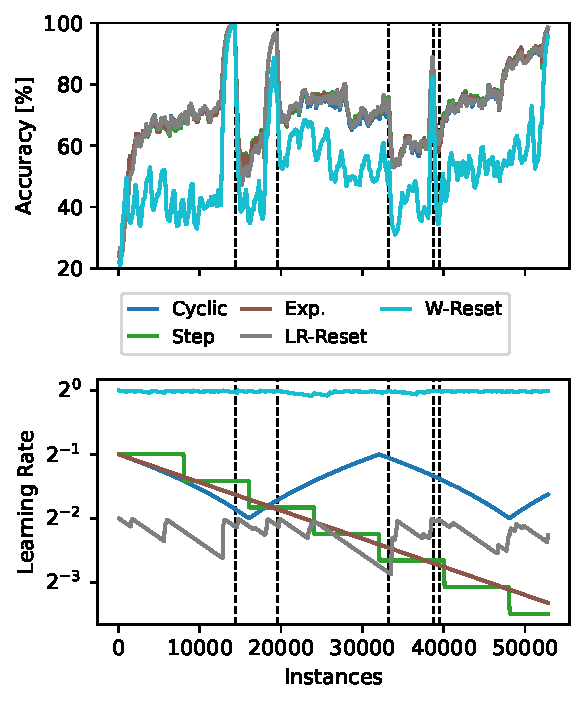
\includegraphics[width=.47\textwidth]{figures/lr_norms_schedules_insects_abrupt.pdf}
	\caption{Prequential accuracy and learning rate for static and drift adaptive  schedules on \textit{Insects abrupt} dataset. Concept drifts are marked by dashed lines. Accuracy was exponentially smoothed with a decay factor of 0.75.}
	\label{fig:prequential_schedulers_insects}
\end{figure}

To evaluate the effectiveness of our learning rate resetting mechanism for drift adaptation (see Equation~\eqref{eq:drift_reset}), we compare its average prequential accuracy to that of the adaptation algorithm by \citet{kunchevaAdaptiveLearningRate2008} (see Equation~\eqref{eq:kuncheva_lr}) and model weight resetting, commonly used in online learning.

As can be seen in Table~\ref{tab:lr_resetting}, our approach clearly outperforms both other drift adaptation techniques by a wide margin on all but \textit{Covertype}, where weight resetting yielded slightly higher accuracy.
It also compares favorably against static exponential decay on the \textit{RBF incremental}, \textit{Covertype} and \textit{Electricity} datasets.
However, aside from the results on \textit{RBF incremental} the accuracy increases are negligible.
Furthermore, learning rate resetting did not yield improvements for the Insects datasets regardless of the type of drift.
This is also reflected in Figure~\ref{fig:prequential_schedulers_insects}, where the standard exponential schedule's accuracy initially rises faster and recovers faster after the first concept drift, which is likely caused by its larger step size in the first half of the stream.
Although the resetting mechanism frequently acted when no concept drift occurred, our results for the oracle resetting approach, that was triggered only for timesteps with drift, show that this performance gap is not caused by the drift detector.
Rather, it appears that using a larger initial learning rate and slower decay is sufficient for assuring adequate adaptability to concept drift throughout a data stream while granting better stability at later stages.
Overall, a slower but static decay paired with a larger initial learning rate seems to be preferable over a more aggressive schedule with our drift resetting mechanism, unless severe concept drift as in \textit{RBF incremental} is expected.

With accuracy values within the $1\sigma$ interval of one another on all evaluated streams, step-wise decay displays almost identical performance to exponential decay.
The cyclic schedule's accuracy for \textit{RBF incremental} and \textit{Covertype} on the other hand significantly exceeded that of the other static and adaptive schedules but lacks behind on all other streams.
We also did not find improvements in convergence speed by an order of magnitude as observed by~\cite{smithSuperConvergenceVeryFast2018a} for the investigated scenario.
Based on our results, the usefulness of cyclic learning rates for online learning applications therefore seems to be more data dependent than conventional decaying schedules.

\subsection{Adaptive Learning Rates}

\begin{figure}[ht]
	\centering
	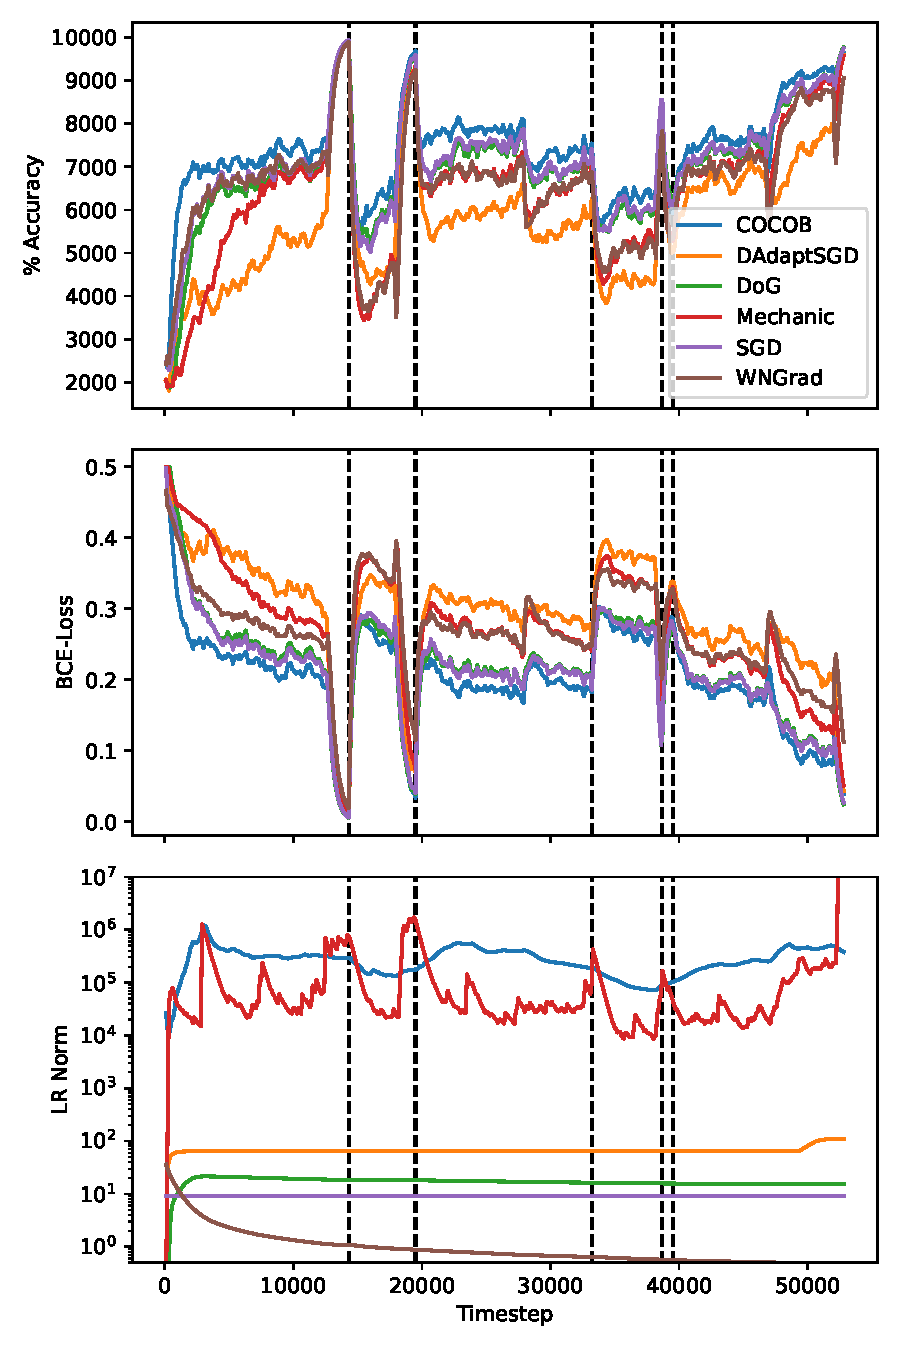
\includegraphics[width=.47\textwidth]{figures/lr_norms_optims_insects_abrupt.pdf}
	\caption{Prequential accuracy and learning rate for adaptive optimizers on \textit{Insects abrupt} dataset. Concept drifts are marked by dashed lines. Accuracy is exponentially smoothed with a decay factor of 0.75.}
	\label{fig:prequential_optims_insects}
\end{figure}
\begin{table*}[ht]
	\centering
	\small
	\begin{tabular}{llcccccccc}
		\toprule
		                                                   & Optimizer & RBF abrupt          & RBF incr.            & Covertype             & Electricity          & Insects abrupt      & Insects gradual     & Insects incr.       \\
		\midrule
		\multirow{5}{*}{\rotatebox[origin=c]{90}{Tuned}}   & SGD       & \bfseries 94.79±.32 & 70.95±2.89           & \bfseries 83.42±.50   & 73.77±.40            & 71.50±.08           & 75.31±.21           & 60.48±.20           \\
		                                                   & Adam      & 93.45±.30           & 69.26±5.14           & 79.01±.27             & 69.79±.54            & \bfseries 75.38±.24 & 75.78±.74           & \bfseries 64.17±.13 \\
		                                                   & AdaGrad   & 92.45±1.37          & 52.87±6.62           & 81.68±.35             & \bfseries 76.99±1.20 & 74.87±.40           & \bfseries 77.15±.27 & 62.51±.59           \\
		                                                   & WNGrad    & 87.30±.68           & 44.92±.73            & 76.98±.15             & 70.80±.59            & 66.25±.19           & 66.75±.40           & 56.14±.21           \\
		                                                   & HD        & 93.92±.31           & \bfseries 72.29±2.90 & \underline{83.36±.25} & 73.83±.32            & 70.67±.06           & 73.37±.21           & 59.92±.18           \\ \midrule
		\multirow{4}{*}{\rotatebox[origin=c]{90}{LR-Free}} & COCOB     & \bfseries 93.40±.38 & 63.52±2.70           & 82.27±.46             & \bfseries 84.30±.56  & \bfseries 74.75±.11 & \bfseries 77.00±.05 & \bfseries 63.65±.16 \\
		                                                   & DoG       & 92.72±.59           & \bfseries 73.17±2.72 & \bfseries 83.07±.64   & 71.53±.70            & 70.59±.26           & 74.01±.21           & 59.66±.22           \\
		                                                   & D-Adapt   & 74.91±4.22          & 45.47±2.75           & 76.69±.79             & 66.03±1.75           & 50.05±11.26         & 48.21±10.62         & 36.00±11.81         \\
		                                                   & Mechanic  & 88.94±.58           & 49.26±1.44           & 78.67±.18             & 50.73±7.60           & 55.31±21.47         & 65.80±.53           & 47.89±17.46         \\
		\bottomrule
	\end{tabular}
	\caption{Average prequential accuracy [\%] for adaptive optimizers and SGD. We used SGD as the base optimizer for HD, Mechanic and D-Adapt. Best values are shown in \textbf{bold}, values within $1\sigma$ interval of best values are \underline{underlined}.}
	\label{tab:results_adaptive_optims}
\end{table*}

To judge the usefulness of different adaptive first-order optimization techniques for online learning, we ran prequential evaluations with all methods listed in Table~\ref{tab:param_free_optims}.

From the results displayed in Table~\ref{tab:results_adaptive_optims}, it can be deduced that none of the approaches that require tuning a step size parameter stands out as generally superior for the investigated datasets.
Rather, each of SGD, AdaGrad, and Adam achieve the best accuracy on two of the seven datasets.
This once again underlines the data dependency of the optimizer performance.
However, since SGD yields the best accuracy on \textit{RBF abrupt} but is clearly surpassed on \textit{Insects abrupt}, the type of concept drift does not seem to be significant.

Due to its simplicity and favorable computational efficiency, it appears that standard SGD should be selected out of the non-parameter-free approaches if the characteristics of the targeted data stream are unknown.
The SGD variant of Hypergradient Descent (HD)~\cite{baydinOnlineLearningRate2018} and WNGrad~\cite{wuWNGradLearnLearning2020} on the other hand seem to rarely be optimal choices.

In the category of learning rate free optimizers COCOB~\cite{orabonaTrainingDeepNetworks2017}, outperformed its competitors on all but two datasets.
It comes close to or even exceeds the best tuned approaches in terms of accuracy.
Although yielding lower accuracy on average, DoG also comes within reach of the tuned methods, while offering much better runtime and memory efficiency compared to COCOB (see Table~\ref{tab:param_free_optims}).
Mechanist~\cite{cutkoskyMechanicLearningRate2023} and D-Adaptation~\cite{defazioLearningRateFreeLearningDAdaptation2023a}, which we ran with SGD as the base optimizer performed significantly worse than their competitors on the evaluated streams.

To gain additional insights into the investigated adaptive optimizers, we calculated their effective learning rates as $\frac{||\eta_t||}{\sqrt{D}}$, where $\eta_t \in \mathbb{R}^D$ is the vector of parameter specific learning rates.
The resulting learning rate curves shown in Figure~\ref{fig:prequential_schedulers_insects}, provide an indication regarding the reason for the poor performance of WNGrad and D-Adaption.
Whereas the learning rate of DoG quickly approaches the tuned SGD learning rate, the two parameter-free methods diverge considerably from it.
A possible cause for this could be the higher level of gradient noise introduced by the small mini-batches and concept drift associated with data streams.

Another interesting observation in Figure~\ref{fig:prequential_optims_insects} is that the learning rate of the best performing Adam features spikes for most change points, suggesting some form of adaptability to drift.
Since the much worse performing Mechanic shows similar spikes, this is however unlikely to be a significant contributing factor to Adam's high accuracy on \textit{Insects abrupt}. 
Instead, it likely stems from its second moment scaling, which is also part of the similarly performing AdaGrad.

It may also be noted that the learning rates of the COCOB, Adam and Mechanic optimizers with parameter specific learning rates exceed those of single value step sizes by multiple orders of magnitude.
This is an effect of second moment scaling, which creates larger learning rates for parameters with small and consistent gradients~\cite{cutkoskyMechanicLearningRate2023}.
Therefore, the parameter updates generated by these approaches are not necessarily larger.

\subsection{Learning Rate Tuning}

\begin{figure}[ht]
	\centering
	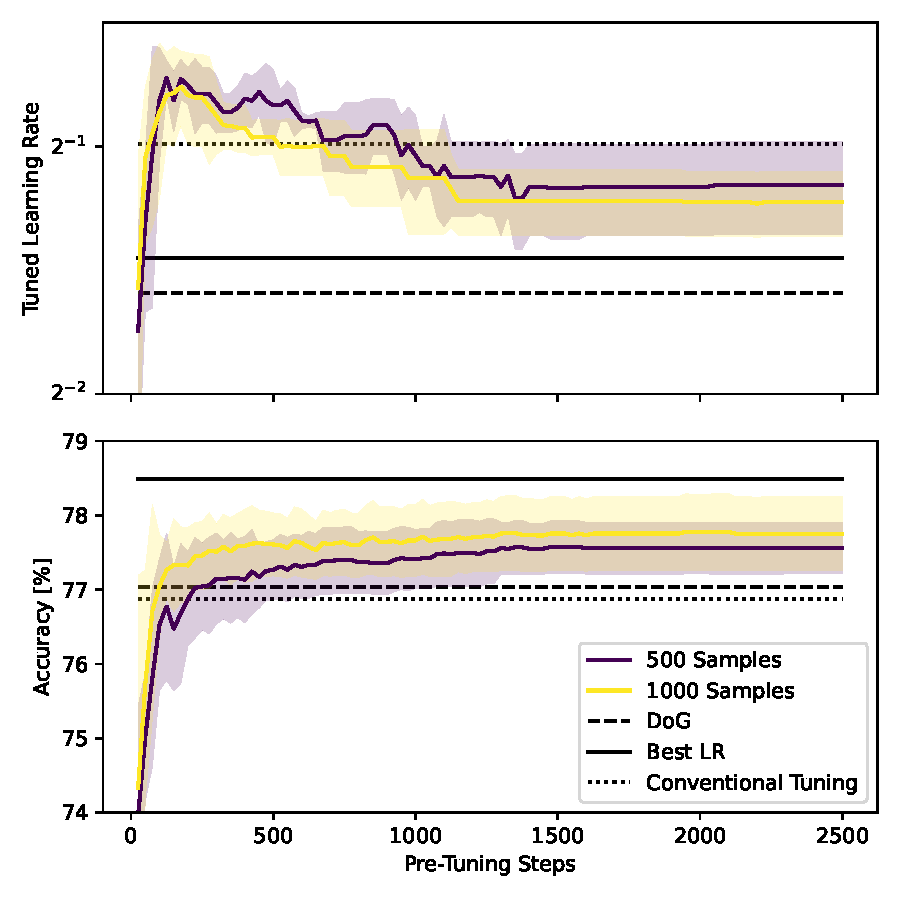
\includegraphics[width=.45\textwidth]{figures/pretune_1x64_acc_lr_exp_schedule.pdf}
	\caption{Pre-tuned LR (LR that maximizes accuracy on pre-tuning data) and resulting accuracy on data streams when using SGD and an exponential learning rate schedule with 500 or 1000 separate tuning samples. Results are averaged over all real-world datasets. The shaded area represents the 1$\sigma$-interval.}\label{fig:pretune_lr_accuracy}
\end{figure}

We assessed our suggested approach of pre-tuning learning rates for MLPs with 64 or 128 hidden units per layer and either one or three hidden layers.
In the following part, we focus on the smallest network that is the most representative for streaming applications.
The results of all architectures are reported in Appendix~\ref{app:pretune_model_sizes}.

Prequential evaluation runs were performed with a range of initial learning rates $\eta_0$ and exponential decay factors $\gamma$.
From each data stream, we select a subset of either 500 or 1000 instances at the beginning by holding them out from the remaining data.
In the pre-tuning process, we then bootstrap samples from the held out data to emulate a stream and determine the learning rate yielding the best mean prequential accuracy at each step.
We use accuracy instead of loss as the selection criterion, because the binary crossentropy employed for training commonly decreases by orders of magnitude throughout optimization.
A selection based on the prequential loss would therefore only consider the initial iterations of the tuning process.

Figure~\ref{fig:pretune_lr_accuracy} shows the learning rate resulting from the pre-tuning process at each tuning step averaged over all real-world datasets.
The bottom row of the figure displays the mean accuracy achieved when using this learning rate on the remaining data stream not used for tuning.

After overshooting initially, the tuned learning rate converges in the vicinity of optimal learning rate after 1000 iterations.
While tuning with 1000 samples yields a better approximation of the optimal value, both subset sizes on average achieve significantly better learning rates for more than 1000 pre-tuning steps, than conventional tuning performed with 800 training and 200 validation samples.
This is also reflected in the accuracy scores, which exceed conventional tuning after 500 iterations.
Our approach achieves notably higher accuracy than DoG, which we selected as a baseline due to being best performing parameter-free optimizer with a global learning rate.
This is the case despite deviating further from the optimal learning rate, likely due to excessively low learning rates having a larger impact than excessively high ones in the evaluated scenario.

% Figure~\ref{fig:pretune_fixed_vs_exp_lr} shows that when provided with sufficient data, pre-tuning also significantly outperforms DoG for a fixed learning rate.
% However, its performance benefit compared to DoG is considerably larger with a decaying schedule.

In conclusion, our proposed tuning approach enables significantly better learning rate selection for prequential evaluation on data streams compared to both conventional tuning and DoG.
Additionally, pre-tuning has the benefit that once completed, no additional memory or runtime costs are incurred.
In streaming applications, where computing resources are often times a limiting factor, this could be a critical advantage.
Although, if computational efficiency is insignificant, the highly performant but expensive COCOB~\cite{orabonaTrainingDeepNetworks2017} or the slightly less performant and much less expensive DoG~\cite{ivgiDoGSGDBest2023} may be more appropriate.

% \begin{figure}[ht]
% 	\centering
% 	\begin{tikzpicture}
% 		% Upper image
% 		\node[inner sep=0pt] (upper) {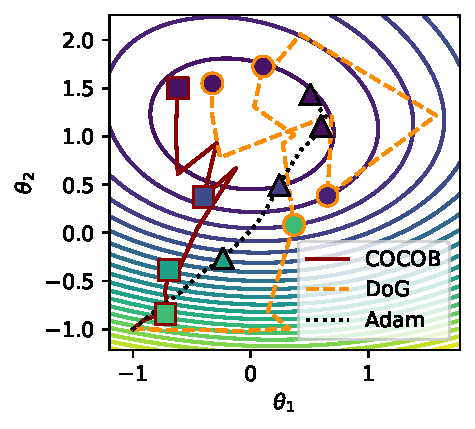
\includegraphics[width=0.4\textwidth]{figures/sgd_trajectory_optims1.pdf}};

% 		% Lower image
% 		\node[inner sep=0pt, below=3mm of upper] (lower){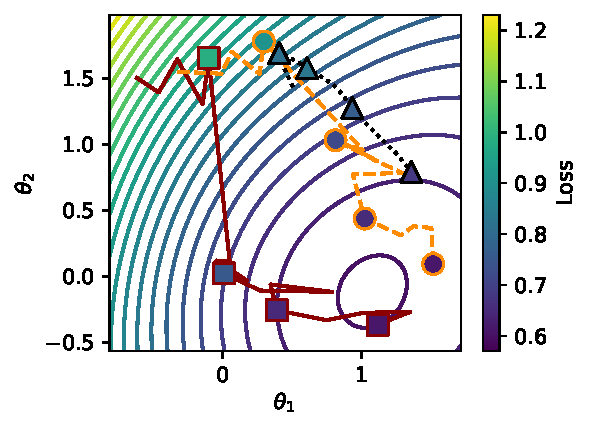
\includegraphics[width=0.4\textwidth]{figures/sgd_trajectory_optims2.pdf}};

% 		\path ([xshift=-8pt]upper) -- ([xshift=-8pt]lower) node[midway] (text){Concept Drift};
% 		\draw[->] ([xshift=-5pt, yshift=5pt]upper.south-|text.west) -- ([xshift=-5pt, yshift=-3pt]lower.north-|text.west);
% 		\draw[->] ([xshift=5pt, yshift=5pt]upper.south-|text.east) -- ([xshift=5pt, yshift=-3pt]lower.north-|text.east);

% 	\end{tikzpicture}
% 	\caption{Parameter trajectory of COCOB~\cite{orabonaTrainingDeepNetworks2017}, DoG~\cite{ivgiDoGSGDBest2023} and Adam~\cite{kingmaAdamMethodStochastic2017b} on synthetic data stream with abrupt concept drift. Marker colors depict the expected prequential loss over the last 16 data instances.}
% \end{figure}

\section{Conclusion}

In this work, we investigate the influence and selection of the learning rate and optimization procedure with respect to deep learning in streaming environments.
We first provide theoretical background on discrepancies between learning rate optimization in conventional batch learning and online learning.
Based on these differences, we derive a simple mechanism resetting the learning rate on concept drift occurrences.
We then give an overview learning rate free algorithms popular in batch learning, which we compare experimentally on multiple synthetic and real-world datasets,
finding both COCOB and DoG to come close to the performance of optimizers with tuned learning rates.
Lastly, we introduce a streaming specific learning rate tuning approach that grants significant performance increases over conventional tuning via a train-validation split.

% \clearpage

\bibliography{aaai24}
% \newpage
\appendix

\section{Hyperparameter values}\label{app:hyperparams}

In our experiments we used the following hyperparameter settings.

\begin{table}[H]
	\centering
	\begin{tabular}{ll}
		\toprule
		Schedule    & Static                            \\ \midrule
		Exponential & $\gamma=1-2^{-13}$                \\
		Exp. Reset  & $\gamma=1-2^{-12}, \delta=0.0001$ \\
		Step        & $\gamma=0.75, s=2000$             \\
		Cyclic      & $\hat{\eta}=0.25, s=8000$         \\ \bottomrule
	\end{tabular}
	\caption{Learning Rate Schedule Hyperparameters.}
\end{table}

\begin{table}[H]
	\centering
	\begin{tabular}{ll}
		\toprule
		Optimizer  & Learning Rate                                  \\
		\midrule
		SGD        & $\{2^{1}, 2^{0}, \ldots, 2^{-8}\}$             \\
		Adam       & $\{2^{-3}, 2^{-4}, \ldots, 2^{-12}\}$          \\
		AdaGrad    & $\{2^{1}, 2^{0}, \ldots, 2^{-8}\}$             \\
		WNGrad     & $\{10^{1.25}, 10^{0.75}, \ldots, 10^{-7.75}\}$ \\
		SGD-HD     & $\{2^{-3}, 2^{-4}, \ldots, 2^{-12}\}$          \\ \midrule
		COCOB      & $100$                                          \\
		DoG        & $1$                                            \\
		D-AdaptSGD & $1$                                            \\
		Mechanic   & $0.01$                                         \\
		\bottomrule
	\end{tabular}
	\caption{Search spaces for learning rates of different optimizers.}
\end{table}

\newpage

\section{Learning Rate Pre-Tuning Results}\label{app:pretune_model_sizes}

% \begin{figure}[]
% 	\centering
% 	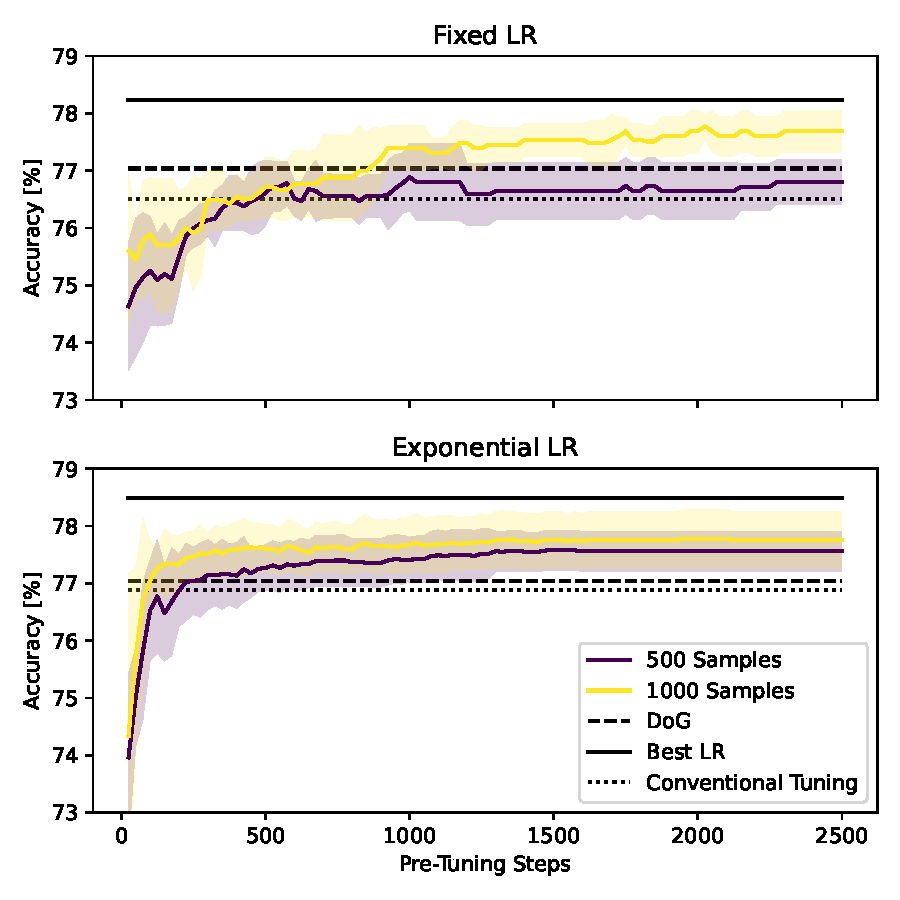
\includegraphics[width=.47\textwidth]{figures/pretune_1x64_fixed_vs_exp_schedule.pdf}
% 	\caption{Accuracy achieved by pre-tuning on 500 or 1000 samples when using SGD with a fixed LR schedule (top) or an exponential schedule (bottom), averaged over all real-world datasets. The shaded area represents the 1$\sigma$-interval.}\label{fig:pretune_fixed_vs_exp_lr}
% \end{figure}

\begin{figure}[h]
	\centering
	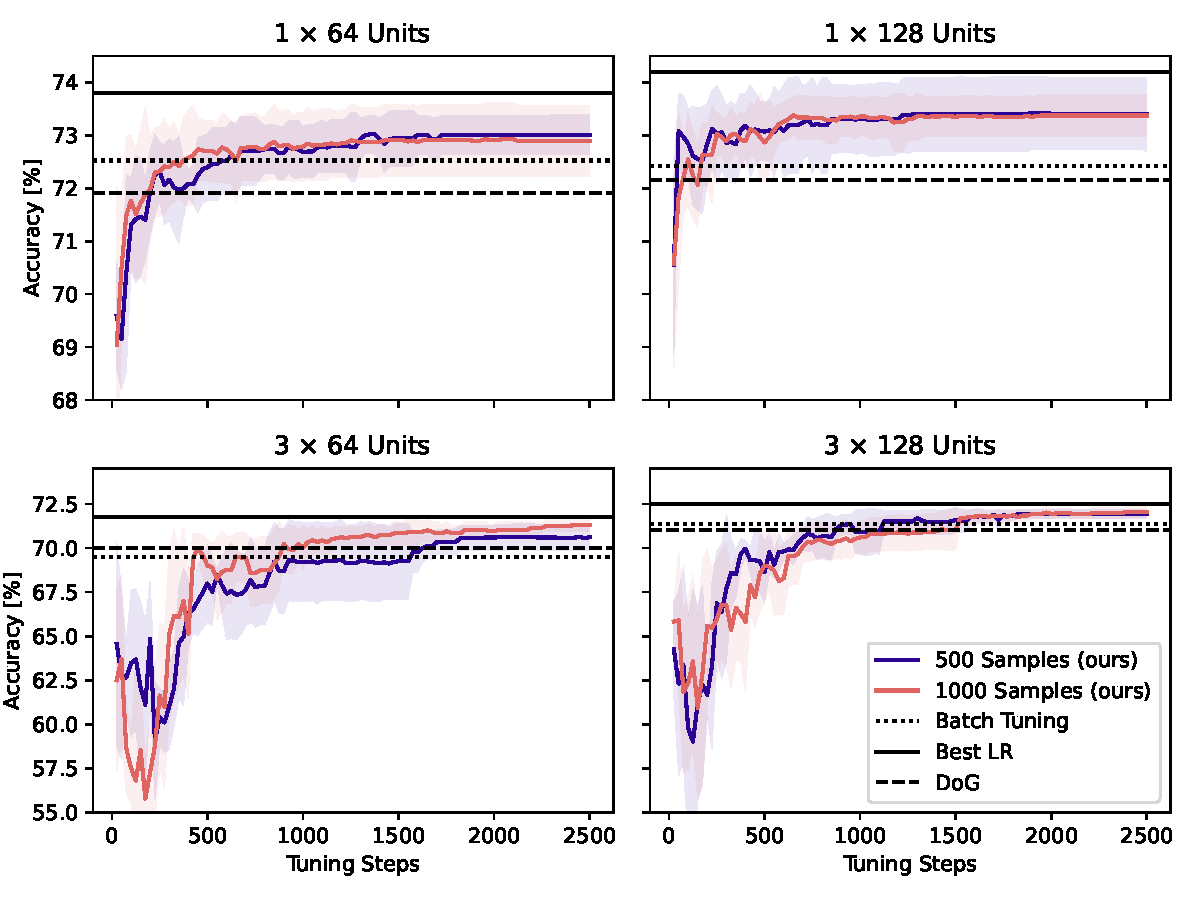
\includegraphics[width=.47\textwidth]{figures/pretune_architectures_exp_schedule.pdf}
	\caption{Accuracy achieved by pre-tuning on 500 or 1000 samples when using SGD with an exponential schedule on different network sizes, averaged over all real-world datasets. The shaded area represents the 1$\sigma$-interval.}
\end{figure}

\end{document}
